\chapter{Analyse des besoins et identification des use cases}
\section{Approche SCAN -- PLAN -- ACT}
La démarche d'identification des besoins a consisté à passer d'une observation générale du domaine WMS vers des use cases traçables. La figure~\ref{fig:scan-plan-act} synthétise cette progression.

\begin{figure}[H]
\centering
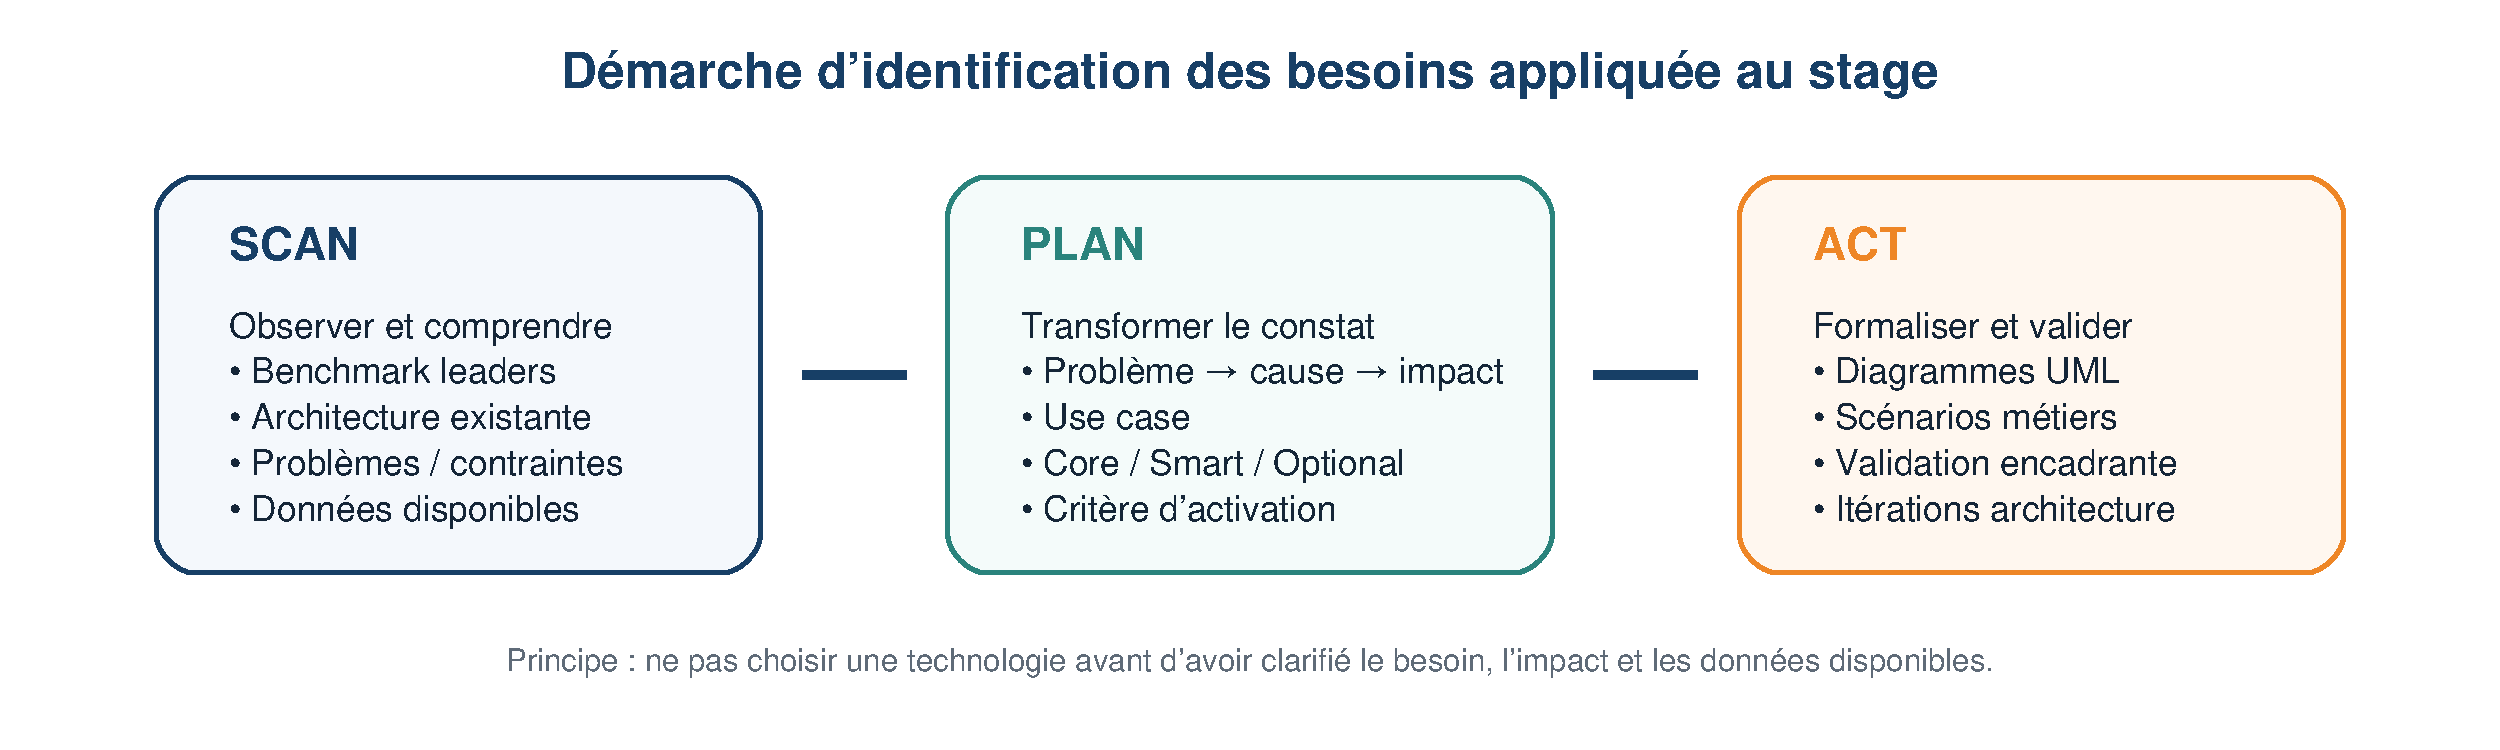
\includegraphics[width=0.92\linewidth]{figures/chapitre3/demarche_scan_plan_act.pdf}
\caption{Application de la démarche SCAN -- PLAN -- ACT à l'identification et à la validation des besoins.}
\label{fig:scan-plan-act}
\end{figure}

\section{Logique de classification}
La classification Core / Smart / Optional évite de confondre une fonction indispensable avec une capacité avancée ou dépendante d'une infrastructure. Le Core correspond aux capacités nécessaires au fonctionnement du WMS. Le Smart améliore la décision grâce aux données, à l'optimisation ou au machine learning. L'Optional dépend d'un équipement ou d'un système particulier : caméra 3D, RFID, AMR/AGV, WCS/WES ou BMS/EMS.

\begin{figure}[H]
\centering
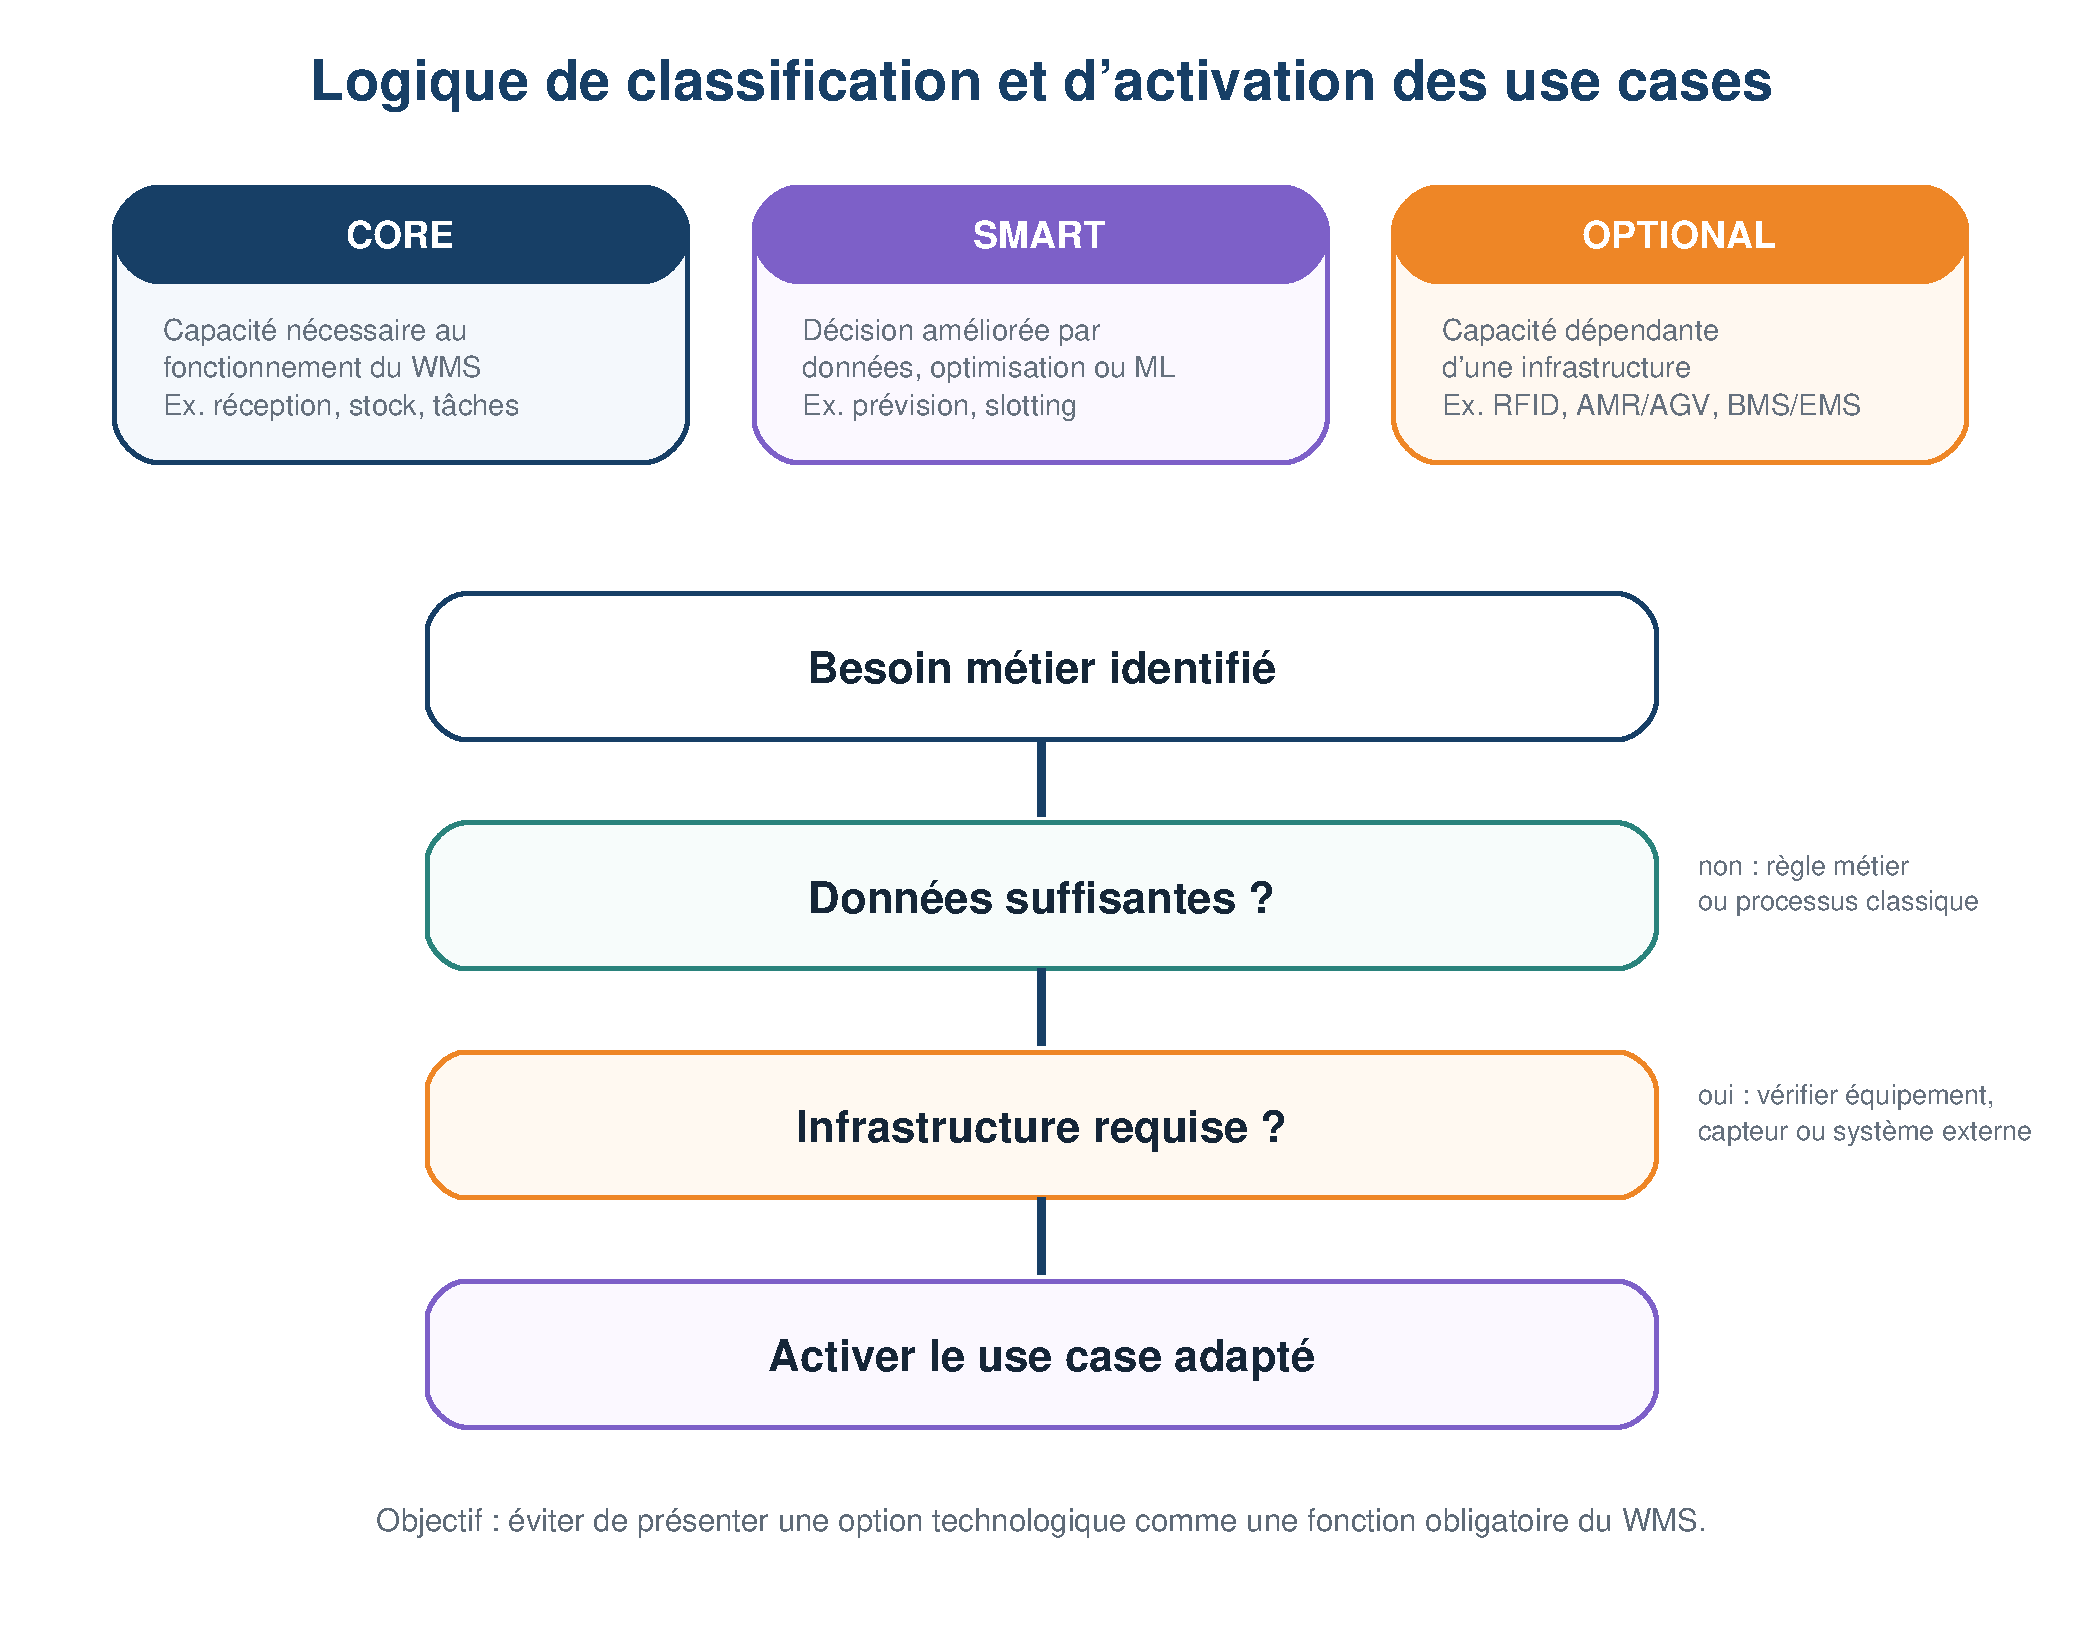
\includegraphics[width=\linewidth]{figures/chapitre3/classification_activation.pdf}
\caption{Logique Core / Smart / Optional et principe d'activation selon les données et l'infrastructure.}
\label{fig:classification}
\end{figure}

\section{Cartographie des use cases}
Les tableaux suivants conservent la numérotation validée pendant le stage.

\begin{longtable}{p{2.2cm}p{9.2cm}p{3cm}}
\caption{Use cases Réception}\\
\toprule
ID & Use case & Type \\
\midrule
UC-R01 & Planifier rendez-vous et quai & Core \\
UC-R02 & Réceptionner les marchandises & Core \\
UC-R03 & Identifier le produit & Core \\
UC-R04 & Contrôler la quantité & Core \\
UC-R05 & Contrôler la qualité & Core \\
UC-R06 & Gérer une anomalie de réception & Core \\
UC-R07 & Proposer emplacement de stockage & Core \\
UC-R08 & Prévoir la charge de réception & Smart \\
UC-R09 & Compter les cartons par caméra 3D & Optional \\
UC-R10 & Lire l'étiquette par OCR & Optional \\
UC-R11 & Détecter les défauts par vision & Optional \\
UC-R12 & Suivre le conteneur connecté & Optional \\
\bottomrule
\end{longtable}

\begin{longtable}{p{2.2cm}p{9.2cm}p{3cm}}
\caption{Use cases Stockage et Inventaire}\\
\toprule
ID & Use case & Type \\
\midrule
UC-S01 & Mettre en stock / putaway & Core \\
UC-S02 & Gérer les stocks & Core \\
UC-S03 & Gérer les emplacements & Core \\
UC-S04 & Réaliser l'inventaire tournant & Core \\
UC-S05 & Réapprovisionner la zone picking & Core \\
UC-S06 & Détecter la congestion d'une zone & Smart \\
UC-S07 & Surveiller les produits sensibles & Core conditionnel \\
UC-S08 & Gérer lots / DLC / FEFO & Core conditionnel \\
UC-S09 & Choisir l'emplacement optimal / slotting & Smart \\
UC-S10 & Cibler les emplacements à recompter & Smart \\
UC-S11 & Prédire une rupture avant blocage & Smart \\
UC-S12 & Chercher un emplacement alternatif & Smart \\
UC-S13 & Suivre les palettes par RFID & Optional \\
UC-S14 & Déplacer le stock par AMR / AGV & Optional \\
\bottomrule
\end{longtable}

\begin{longtable}{p{2.2cm}p{9.2cm}p{3cm}}
\caption{Use cases Commandes et Expédition}\\
\toprule
ID & Use case & Type \\
\midrule
UC-E01 & Recevoir la commande client & Core \\
UC-E02 & Planifier la commande & Core \\
UC-E03 & Créer la wave / batch & Core \\
UC-E04 & Allouer le stock & Core \\
UC-E05 & Créer tâches de picking & Core \\
UC-E06 & Effectuer le picking & Core \\
UC-E07 & Effectuer le packing & Core \\
UC-E08 & Charger le camion & Core \\
UC-E09 & Expédier la commande & Core \\
UC-E10 & Guider le picking RF / Pick-to-Light & Optional \\
UC-E11 & Optimiser le parcours picking & Smart \\
UC-E12 & Contrôler le picking scan / poids / vision & Optional \\
UC-E13 & Recommander l'emballage & Smart \\
UC-E14 & Contrôler le chargement scan / caméra & Optional \\
UC-E15 & Détecter commandes à risque de retard & Smart \\
\bottomrule
\end{longtable}

\begin{table}[H]
\centering
\caption{Synthèse des catégories et critères d'activation par domaine}
\begin{tabularx}{\linewidth}{p{3cm}X X X}
\toprule
Domaine & Core & Smart & Optional / infrastructure \\
\midrule
Réception & UC-R01--UC-R07 & UC-R08 & UC-R09--UC-R12 \\
Stockage & UC-S01--UC-S05, UC-S07--UC-S08 & UC-S06, UC-S09--UC-S12 & UC-S13--UC-S14 \\
Commandes & UC-E01--UC-E09 & UC-E11, UC-E13, UC-E15 & UC-E10, UC-E12, UC-E14 \\
Yard & UC-Y01--UC-Y04 & UC-Y06--UC-Y07 & UC-Y05 \\
Ressources & UC-RES01--03, UC-RES05--06, UC-RES08 & UC-RES04 & UC-RES07, UC-RES09--10 \\
\bottomrule
\end{tabularx}
\end{table}
